\documentclass{llncs}

\pagestyle{headings}

%\usepackage{showkeys}
\usepackage{hyperref}
\usepackage{url}
\usepackage{relsize}
\usepackage{amsmath}
\usepackage{amssymb}
\usepackage{stmaryrd}
\usepackage{graphicx}
\usepackage[T1]{fontenc}
\usepackage{listings, framed}
\usepackage[dvipsnames]{xcolor}
\usepackage{orcidlink}

% \|name| or \mathid{name} denotes identifiers and slots in formulas
\def\|#1|{\mathid{#1}}
\newcommand{\mathid}[1]{\ensuremath{\mathit{#1}}}
% \<name> or \codeid{name} denotes computer code identifiers
\def\codesize{\small}
\def\<#1>{\codeid{#1}}
\newcommand{\codeid}[1]{\ifmmode{\mbox{\codesize\ttfamily{#1}}}\else{\codesize\ttfamily #1}\fi}

\renewcommand{\exp}{\mathit{exp}}
\newcommand{\com}{\mathit{com}}
\newcommand{\aop}[2]{{#1}\ \mathit{aop}\ {#2}}
\newcommand{\field}[2]{{#1}\mathtt{.}{\mathit{#2}}}
\newcommand{\size}[1]{{#1}\mathtt{.size()}}
\newcommand{\random}[1]{\mathtt{random(}{#1}\mathtt{)}}
\newcommand{\last}[1]{{#1}\mathtt{.last()}}
\newcommand{\new}[2]{\mathtt{new}\ \mathit{#1}\mathtt{(}{#2}\mathtt{)}}
\newcommand{\call}[3]{{#1}\mathtt{.}{#2}\mathtt{(}{#3}\mathtt{)}}
\newcommand{\readmap}[3]{{#1}\mathtt{[}{#2}\mathtt{]\ else\ }{#3}}
\newcommand{\writemap}[3]{{#1}\mathtt{[}{#2}\mathtt{]:=}{#3}}
\newcommand{\push}[2]{{#1}\mathtt{.push(}{#2}\mathtt{)}}
\newcommand{\receive}[2]{{#1}\mathtt{.receive(}{#2}\mathtt{)}}
\newcommand{\require}[2]{\mathtt{require(}{#1}\ \mathit{cop}\ {#2}\mathtt{)}}
\newcommand{\assign}[2]{{#1}\mathtt{:=}{#2}}
\newcommand{\ife}[4]{\mathtt{if\ (}{#1}\ \mathit{cop}\ {#2}\mathtt{)\ then\ }{#3}\mathtt{\ else\ }{#4}}
\newcommand{\ifetwo}[4]{\begin{array}{l}
    \mathtt{if\ (}{#1}\ \mathit{cop}\ {#2}\mathtt{)}\\
    \mathtt{\ then\ }{#3}\mathtt{\ else\ }{#4}
\end{array}}
\newcommand{\for}[3]{\mathtt{for\ }{#1}\mathtt{\ in\ }{#2}\ {#3}}
\newcommand{\sequence}[2]{{#1}\mathtt{;}{#2}}
\newcommand{\da}[2]{\mathbb{DA}_{{#1}}\left\llbracket{#2}\right\rrbracket}
\newcommand{\dastates}[1]{\mathsf{DA}_{{#1}}}
\newcommand{\paths}[1]{\mathsf{P}_{{#1}}}
\newcommand{\relevantpaths}[1]{\mathsf{RP}_{{#1}}}

\newcommand{\todo}[1]{{\color{red}\bfseries [[#1]]}}
\newcommand{\wrt}{\textit{wrt.\ }}
\newcommand{\ie}{, \textit{ie.}, }
\newcommand{\ieinitial}{\textit{ie.}, }

\newcommand{\sideeffect}[2]{\mathsf{se}_{{#1}}\mathsf{(}{#2}\mathsf{)}}
\newcommand{\dom}{\mathit{dom}}
\newcommand{\pair}[2]{\langle{#1},{#2}\rangle}
\newcommand{\unchanged}{\mathit{unchanged}}
\newcommand{\survives}[1]{\xrightarrow{{#1}}}
\newcommand{\nat}{\mathbb{N}}
\newcommand{\res}{\mathit{res}}
\newcommand{\val}{\mathit{value}}
\newcommand{\length}{\mathit{len}}
\newcommand{\lfp}{\mathit{lfp}}

\lstdefinelanguage{pseudo}{
        keywords=[1]{assert, break, case, catch, class, final, continue, default, do, else, extends, false, finally, for, if, implements, import, instanceof, interface, new, private, 
protected, public, static, payable, return, super, switch, this, throw, throws, true, try, var, while,in }, % generic keywords including crypto operations
        keywordstyle=[1]\color{blue}\bfseries,
        keywords=[2]{Contract, PayableContract, List, int, float, double, short, byte, long, boolean, void, String},
        keywordstyle=[2]\color{teal}\bfseries,
        keywords=[3]{this, caller, amount, now},
        keywordstyle=[3]\color{violet}\bfseries,
        keywords=[4]{push, require, receive, size, random},
        keywordstyle=[4]\color{red}\bfseries,
        identifierstyle=\color{black},
        sensitive=true,
        comment=[l]{//},
        morecomment=[s]{/*}{*/},
        commentstyle=\color{gray}\ttfamily,
        stringstyle=\color{red}\ttfamily,
        morestring=[b]',
        morestring=[b]"
}

\lstset{ % define general preferences
        language=pseudo,
        %backgroundcolor=\color{verylightgray},
        extendedchars=true,
        basicstyle=\scriptsize\ttfamily,
        showstringspaces=false,
        showspaces=false,
        numbers=left,
        numberstyle=\scriptsize,
        numbersep=5pt,
        tabsize=2,
        breaklines=true,
        showtabs=false,
        captionpos=b,
        escapeinside={||},
}

\begin{document}

\begin{frontmatter}

  \title{Boundness Analysis for Smart Contracts}

  \author{
    Fausto Spoto\orcidlink{0000-0003-2973-0384}
  }
  \institute{
    Dipartimento di Informatica, Universit\`a di Verona, Italy\\
    \email{fausto.spoto@univr.it}
  }

  \maketitle

  \begin{abstract}
    This is the abstract.
  \end{abstract}

\end{frontmatter}

\pagenumbering{arabic}

\section{Introduction}\label{sec:introduction}

Smart contracts are computer programs that get executed
inside the nodes of a blockchain network. They express some form of
agreement among parties, that gets enforced by the properties of the
underlying
blockchain. Namely, the blockchain's data immutability and its consensus
algorithm make it hard
to violate the rules of the protocol, replace data
or censure specific transactions.
While this is desirable for protocols that must hold
and resist in the wild, it also means that code bugs, if present,
are also enforced and cannot be patched.
Therefore, it is highly relevant to deploy smart contracts
only if they do not contain software bugs.
There is large literature about bugs that led to
protocol breaches and stolen money (just for the case of Ethereum,
see for instance~\cite{AntonopoulosW25}).
The always cited example of reentrancy shows that attacks to
smart contracts can actually be rather involved and exploit
misunderstood features of the programming language.
In general, the use of Turing-complete programming languages
for writing smart contracts is welcome, but increases the risk
of writing buggy code and lose money. The use of
new programming languages, sometimes with vague or misleading semantics,
further complicates the programming task.

A source of bugs in smart contracts comes from the completely different
way of interaction \wrt traditional software for desktop computers. Namely,
smart contracts operate in the wild. After deployment, their API can
be called in any order and with any argument. There is no such a thing
as a \emph{correct} or \emph{expected} use of a function: users (and attackers)
may call public functions in any order and with any allowed argument.
In this sense, smart contracts are more similar to old-fashioned
servlets and to general-purpose libraries than to traditional software
for desktop computers. Their development requires a careful analysis of their
API and an extensive use of defensive programming, that should foresee all
possible illegal uses. Not surprisingly, many developers,
often unexperienced juniors who jumped on the promising business
of smart contract development,
got overwhelmed by this complexity. Bugs thrived. Money got lost.

This paper focuses on a specific, frequent bug of smart contracts.
Namely, smart contracts often store data in containers, such as lists,
that can be \emph{arbitrarily large}.
This is fine as long as such containers do not get
iterated. Otherwise, the iteration loop might have an arbitrarily large
gas cost, even larger than the maximal gas cost
allowed for a single smart contract transaction.
If that happens, the iteration always fail for gas exhaustion, which might block
some smart contract functionality and, in some case,
even lock money in the contract, forever. The goal of this paper is
to define a static program analysis that guarantees, automatically,
that there exists a maximal size for iterated containers,
for all possible ways of calling the API of a smart contract.
We call such containers \emph{bounded} and the proposed verification technique
is consequently a \emph{boundedness analysis}. Note that
a specific boundedness analysis
does not necessarily compute the exact gas cost for each API function.
If ever possible, that would be a much more concrete analysis,
in terms of abstract interpretation,
with higher cost, more difficulties
and challenges. Boundedness analysis just guarantees the existence
of a bound for the iterated containers. It is up to the programmer
to verify that that bound is small enough for the specific blockchain
at hand. In this sense, boundedness analysis remains blockchain-agnostic.

The specific boundedness analysis defined in this paper
is a sound analysis based on
an abstract interpretation of the trace semantics of the public API
of the smart contract into a set of linear constraints that express
the size change of the iterated containers. Such constraints are
subsequently fed into a theorem prover, that tries to establish
if a maximal bound
exists for the containers. The soundness guarantee is that,
if the theorem prover finds that bound, then
the code does not suffer from boundedness bugs.

The contributions of this paper are:
%
\begin{enumerate}
\item a formal definition of the boundedness property for iterated containers;
\item a sound boundedness analysis, based on abstract interpretation;
\item a prototype implementation for a minimalistic smart contract language.
\end{enumerate}

\begin{figure}[b]
  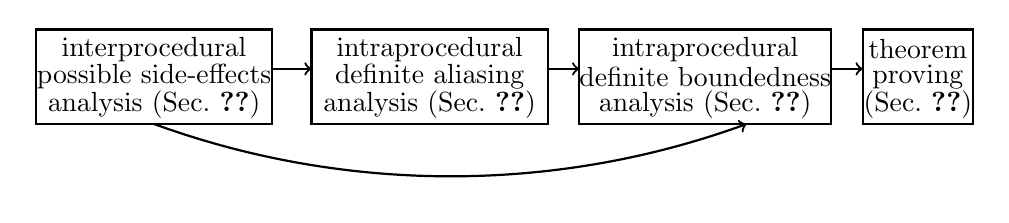
\begin{tikzpicture}
    \draw [thick] (0,0) rectangle +(3,1.2);
    \draw (1.5,0.95) node{interprocedural};
    \draw (1.5,0.6) node{possible side-effects};
    \draw (1.5,0.25) node{analysis (Sec.~\ref{sec:side_effect})};

    \draw[->,thick] (3,0.7) -- +(0.5,0);
    \draw[->,thick] (1.5,0) arc (250:290:11);

    \draw [thick] (3.5,0) rectangle +(3,1.2);
    \draw (5,0.95) node{intraprocedural};
    \draw (5,0.6) node{definite aliasing};
    \draw (5,0.25) node{analysis (Sec.~\ref{sec:aliasing})};

    \draw[->,thick] (6.5,0.7) -- +(0.4,0);

    \draw [thick] (6.9,0) rectangle +(3.2,1.2);
    \draw (8.5,0.95) node{intraprocedural};
    \draw (8.5,0.6) node{definite boundedness};
    \draw (8.5,0.25) node{analysis (Sec.~\ref{sec:boundedness})};

    \draw[->,thick] (10.1,0.7) -- +(0.4,0);

    \draw [thick] (10.5,0) rectangle +(1.4,1.2);
    \draw (11.2,0.95) node{theorem};
    \draw (11.2,0.6) node{proving};
    \draw (11.2,0.25) node{(Sec.~\ref{sec:theorem_prover})};

    %\draw [fill=VioletRed, thick] (0,3.5) rectangle (4,5.5);
  \end{tikzpicture}
  \caption{The components of our boundedness analysis and their dependencies.}
  \label{fig:plan}
\end{figure}

Fig.~\ref{fig:plan} shows the dependencies of the various components of our
boundedness analysis. A preliminary side-effect analysis identifies which lists
might be modified by the execution of the commands. This information is used in
a subsequent aliasing analysis. Both are then used for the actual boundedness analysis,
whose results are sent to a theorem prover, that uses them to prove that there is
no boundedness bug in the program.

The rest of the paper is organized as follows.
Sec.~\ref{sec:examples} presents examples of bounded and unbounded containers
in actual smart contracts, and the potential attacks in case of unboundedness.
Sec.~\ref{sec:syntax} presents the syntax of a minimalistic language for
smart contracts.
Sec.~\ref{sec:side_effect} and \ref{sec:aliasing} define the supporting
side-effect ans aliasing analysis, respectively.
Sec.~\ref{sec:boundedness} defines the actual boundedness
analysis that builds on those two supporting analyses.
Sec.~\ref{sec:theorem_prover} shows how the results of the boundedness
analysis is used to generate constraints that are fed into a theorem
prover. Sec.~\ref{sec:implementation} reports preliminary results
with our prototype implementation.
Sec.~\ref{sec:related} discusses related work. Sec.~\ref{sec:conclusion} concludes.

\section{Examples of Boundness Bugs}\label{sec:examples}

\section{Boundedness Analysis}\label{sec:analysis}

\begin{definition}[Expressions and Commands]\label{def:exp_com}
  \emph{Expressions} and \emph{commands} are defined by the following grammar,
  where $c$ is a literal constant of the language, $\mathit{aop}$ is an arithmetic
  operator and $\mathit{cop}$ is a comparison operator:
  \begin{align*}
    \exp::=&\ \mathit{c}\mid\mathit{v}\mid\field{\exp}{f}\mid\aop{\exp}{\exp}\mid\readmap{\exp}{\exp}{\exp}\\
    &\mid\new{C}{\exp^*}\mid\size{\exp}\mid\last{\exp}\mid\random{\exp}\\
    \com::=&\ \assign{\mathit{v}}{\exp}\mid\assign{\field{\exp}{f}}{\exp}\mid\writemap{\exp}{\exp}{\exp}
    \mid\require{\exp}{\exp}\\
    &\mid\push{\exp}{\exp}\mid\receive{\exp}{\exp}\mid\call{\exp}{m}{\exp^*}\\
    &\mid\ife{\exp}{\exp}{\com}{\com}\mid\for{\mathit{v}}{\exp}{\com}\mid\sequence{\com}{\com}
  \end{align*}
  Expressions and commands are silently annotated with the program point $p$ where they occur
  in the source code under analysis\footnote{For instance, a program point might be
  a line number and a character position inside that line,
  by its exact nature is irrelevant here.}. When useful, that annotation is made
  explicit as $\exp\at{p}$ or $\com\at{p}$.
\end{definition}

\begin{definition}[Program]\label{def:program}
  A \emph{program} is a collection of \emph{classes}.
  Each class $C$ has a superclass,
  some \emph{field signatures}, of the form $C.f$,
  and some \emph{methods}, of the form
  $C.m(p_1 t_1,\ldots,p_n t_n)\mathtt{\ \{}\com\mathtt{\}}$,
  where $\com$ is the \emph{body} of the method.
  A class that extends \<Contract>
  (possibly indirectly) is called a \emph{smart contract}.
  A \emph{constructor} is a method named like the class $C$
  that it belongs to.
\end{definition}
%
Fields and methods can have modifiers such as \<public>, \<private>,
\<final> and \<payable>, that we do not introduce formally and have the
usual meaning as, for instance, in Java or Solidity. For simplicity, we
assume that methods do not return any value.

We assume to analyze a statically strongly-typed language. Therefore, each
expression and command will be evaluated in a context (\emph{typing})
that specifies which variables are in scope and which is their type.
This typing is that inferred in the type-checking phase of the compiler.
%
\begin{definition}[Typing]\label{def:typing}
  A type is either \emph{primitive} (such as \<int>, \<boolean> \ldots)
  or a class name $C$. Generic class types (such as lists) are written as
  \<List<t\texttt{>}>, where \<t> is the type of the elements of the list.
  A \emph{typing} $\tau$ is a map from a finite set of variables
  to their static (\ieinitial declared) type. For any
  expression $\exp$, we write $\tau(\exp)$ for its \emph{type according to $\tau$},
  if its computation does not lead to a type error.
\end{definition}
%
The definition of $\tau(\exp)$ is not formalized here, since it is the usual recursive
definition of the type of an expression, used by any strongly-typed language.
We assume that each program point $p$ comes with an associated typing $\tau\at{p}$.
For any expression $\exp\at{p}$, we assume that $\tau\at{p}$ is \emph{correct} for $\exp$\ie the
computation of $\tau\at{p}(\exp)$ succeeds without type errors.
Such $\tau\at{p}$ is for instance that inferred by the compiler at $p$ during type-checking.

Given an expression or command in the program, it is possible to identify
which lists (and more generally,
which data structures) might be affected by the evaluation of the expression
or by the execution of the command.
Previous work has defined precise and complex static analyses for that
(see for instance the aliasing and side-effect analyses in~\cite{SpotoMP10}).
Here, for simplicity and lack of space,
we present a very simple and cheap side-effect analysis that, nevertheless,
is frequently precise enough on simple programs such as smart contracts.
%
\begin{definition}[Side-Effects Analysis]\label{def:side_effect}
  The set of element types of the lists potentially modified during the evaluation of an
  expression or the execution of a command in the program
  is overapproximated by the minimal fixpoint of the following recursive equations:
  %
  \begin{align*}
    \sideeffect{c}&=\sideeffect{v}=\varnothing\\
    \sideeffect{\new{C}{\exp_1,\ldots,\exp_n}}&=\sideeffect{\com}\cup\bigcup\limits_{i=1}^{n}\sideeffect{\exp_i}\\
    &\quad\text{where $\com$ is the body of the constructor}\\
    \sideeffect{\field{\exp}{f}}&=\sideeffect{\exp}\\
    \sideeffect{\aop{\exp_1}{\exp_2}}&=\sideeffect{\exp_1}\cup\sideeffect{\exp_2}\\
    &\quad\text{similarly, recursively, for the other expressions}
  \end{align*}
  \begin{align*}
    \sideeffect{\push{\exp_1}{\exp_2}\at{p}}&=\sideeffect{\exp_2}\cup\{t\}\quad\text{where $\tau\at{p}(\exp_1)=\<List<>t$\<\text{>}>}\\
    \sideeffect{\call{\exp_0}{m}{\exp_1,\ldots,\exp_n}\at{p}}&=\bigcup\limits_{j=1}^k\sideeffect{\com_j}\cup\bigcup\limits_{i=0}^{n}\sideeffect{\exp_i}\\
    &\quad\text{where $\com_1\cdots\com_k$ are the bodies of}\\
    &\quad\text{the methods possibly called at $p$}\\
    \sideeffect{\sequence{\com_1}{\com_2}}&=\sideeffect{\com_1}\cup\sideeffect{\com_2}\\
    \sideeffect{\assign{\mathit{v}}{\exp}}&=\sideeffect{\exp}\\
    &\quad\text{similarly, recursively, for the other commands.}
  \end{align*}
\end{definition}
%
We recall that a method call in object-oriented languages may actually call a subset
$\{M_1,\ldots,M_k\}$ of the redefinitions of its static target method, with bodies $\{\com_1,\ldots,\com_k\}$.
A sound overapproximation of $\{M_1,\ldots,M_k\}$ can always be inferred statically,
as the set of \emph{all} possible redefinitions. More precise analyses exist~\cite{TipP00},
but are probably overkill for minimalistic code such as smart contracts,
that very rarely redefine methods.

A \emph{path} is an expression rooted at a variable in scope, that follows
\<final> field dereferences or list accesses, or is an integer constant.
Paths have a type and a length. A constant $\kappa$ can be used to limit the maximal
length of a path. A relevant path has type list. While paths will be used
to define the definite aliasing analysis, relevant paths will be used in the
subsequent boundness analysis.
%
\begin{definition}[Paths]\label{def:path}
  Given $\kappa\in\nat$, the finite set $\mathbb{P}^\kappa\at{p}$ of the
  \emph{$\kappa$-paths at program point $p$} is the minimal set such that
  \begin{itemize}
  \item if $\kappa\ge 1$ and $v\in\dom(\tau\at{p})$ then $v\in\mathbb{P}^\kappa\at{p}$, it has type $(\tau\at{p})(v)$
    and $\length(v)=1$ (all variables in scope at $p$ are a $1$-path at $p$);
  \item if $\kappa\ge 1$ and $c\in\nat$ then $c\in\mathbb{P}^\kappa\at{p}$, it has type \<int>
    and $\length(c)=1$ (all integer constants are a $1$-path at $p$);
  \item if $\pi\in\mathbb{P}^\kappa\at{p}$ has type $C$ and $\length(\pi)<\kappa$,
    and if $\mathtt{f}$ is a \<final> field of type $t$ defined in class $C$,
    already initialized at $p$,
    then $\pi.f\in\mathbb{P}^\kappa\at{p}$, it has type $t$ and $\length(\pi.f)=\length(\pi)+1$
    (paths can be expanded by \<final> field dereference);
  \item if $\pi\in\mathbb{P}\at{p}$ has type \<List<$t$\texttt{>}> and $\length(\pi)<\kappa$
    then $\pi\<[any]>\in\mathbb{P}^\kappa\at{p}$, it has type $t$ and $\length(\pi\<[any]>)=\length(\pi)+1$
    (paths can be expanded by list access).
  \end{itemize}
  A $\kappa$-path is \emph{relevant} if its type is \<List<$t$\texttt{>}> for some $t$.
  The finite set of all relevant $\kappa$-paths at $p$ is written as $\mathbb{RP}^\kappa\at{p}$. 
\end{definition}
%
For instance, at line~\ref{ponzi1:require} in Fig.~\ref{fig:ponzi1},
$42$ is a $1$-path of type \<int>,
\<this> is a $1$-path of type \<Ponzi1>,
\<amount> is a $1$-path of type \<int>,
\<this.investors> is a $2$-path of type \<List<Contract\texttt{>}> and
\<this.investors[any]> is a $3$-path of type \<Contract>. Among them, only
\<this.investors> is relevant.

The $\kappa$ limit is essential to make our analysis finitely computable, as shown later.
Larger $\kappa$ lead to a more precise analysis,
in principle, but also potentially more expensive.
Therefore, $\kappa$ acts as a lever that selects the desired precision for the
analysis. For simplicity, in the examples that follow,
we assume $\kappa=3$ and just say \emph{relevant}, meaning $3$-relevant.

A path \emph{survives} the execution of some code\ie it keeps its value unchanged,
if it does not access any list that might be modified by that execution. Note how this
definition is simplified by the constraint that paths only dereference
\<final> fields (Def.~\ref{def:path}), which allows one to focus on side-effects on lists only.
%
\begin{definition}\label{def:survival}
  Given $\pi\in\mathbb{P}^\kappa\at{p}$ and an expression $\exp\at{p}$, then
  \emph{$\pi$ survives the evaluation of $\exp$} if, for all prefix $\pi'$ of $\pi$
  (\ieinitial  $\pi=\pi'\ldots$) of type \<List<$t'$\texttt{>}>
  and for all $t''\in\sideeffect{\exp}$, the types
  $t'$ and $t''$ have no common subtype.
  A similar definition states when \emph{$\pi$ survives the execution of a command $\com$}.
\end{definition}
%
For instance, the path $\pi=\<this.investors>$ at
line~\ref{ponzi1:expand} in Fig.~\ref{fig:ponzi1} does not survive the execution
of the command at that line, since $\pi'=\<this.investors>$
has type \<List<Contract\texttt{>}>,
$\{\<Contract>\}=\sideeffect{\<investors.push(caller)>}$
and \<Contract> has a common subtype with itself, obviously.
Instead, the path $\pi=\<last.sales>$ at line~\ref{lottery2:push_round}
survives the execution of the command at that line, since
the only prefix $\pi'$ of $\pi$ of type list is $\pi'=\pi$, of type
\<List<TicketBatchSale\texttt{>}>,
$\{\<Round>\}=\sideeffect{\<rounds.push(last)>}$ and
\<TicketBatchSale> and \<Round> have no common subtype.
All integer constants survive any expression and command.

\begin{definition}[Definite Aliasing Analysis]\label{def:definite_aliasing}
  An \emph{abstract definite aliasing state at $p$} is a map from each variable
  $v\in\dom(\tau\at{p})$
  to a set of paths that are definitely alias of $v$ (\ieinitial they have the same
  value as $v$). The \emph{abstract definite aliasing denotation} of an expression
  or command at program point $p$ is a map that transforms abstract definite aliasing
  pre-states at $p$ to abstract definite aliasing post-states at the program point after
  the expression or command, defined as:
  %
  \begin{align*}
    \da{c}(\sigma)&=\pair{\sigma}{\{c\}}\quad\text{if $\kappa\ge 1$}\\
    \da{v}(\sigma)&=\pair{\sigma}{\sigma(v)}\\
    \da{\field{\exp}{f}}(\sigma)&=\begin{cases}
    \pair{\sigma'}{\{\pi.f\mid\pi\in\val,\ \length(\pi)<\kappa\}} & \text{if $f$ is \<final>}\\
    \pair{\sigma'}{\varnothing} & \text{otherwise}
    \end{cases}\\
    &\quad\text{where $\da{\exp}(\sigma)=\pair{\sigma'}{\val}$}\\
    \da{\aop{\exp_1}{\exp_2}}(\sigma)&=\pair{\sigma_2}{\{\aop{c_1}{c_2}\mid c_1\in\val_1\cap\nat,\ c_2\in\val_2\cap\nat\}}\\
    &\quad\text{where $\da{\exp_1}(\sigma)=\pair{\sigma_1}{\val_1}$}\\
    &\quad\text{and $\da{\exp_2}(\sigma_1)=\pair{\sigma_2}{\val_2}$}
  \end{align*}
\end{definition}

The static analysis infers size change constraints about the containers
reachable from the state of the smart contracts, for each public API
method or constructor of the smart contract. It distinguishes between
pre-state and after-state by using primed variables for the after-state.
\textbf{This is a sort of simplified path-length. The simplifying
  assumptions must be clarified. The idea is that one does not need
  the supporting analyses such as non-cyclicity or sharing, since the
  domain of analysis is very specific and lists are very well encapsulated.}

For the example in Fig.~\ref{fig:ponzi1}, the inferred approximations are:
%
\begin{description}
\item[\<Ponzi1()>:] $\<investors>'=1$
\item[\<invest()>:] $\<investors>'=\<investors>+1$
\end{description}
%
For the esample in Fig.~\ref{fig:ponzi2} they are (\textbf{something about \<balances>? In any case, it is irrelevant for our proof}):
%
\begin{description}
\item[\<Ponzi2()>:] $\<investors>'=1$
\item[\<invest()>:] $\<investors>'=\<investors>+1$
\item[\<withdraw()>:] $\<investors>'=\<investors>$
\end{description}
%
For the example in Fig.~\ref{fig:ponzi3} they are:
%
\begin{description}
\item[\<Ponzi3()>:] $\<investors>'=1$
\item[\<invest()>:] $\<investors><100\wedge\<investors>'=\<investors>+1$
\end{description}
%
For the example in Fig.~\ref{fig:lottery1} they are:
%
\begin{description}
\item[\<Lottery1()>:] $\<rounds>'=1\wedge\<rounds[any].sales>'=0$
\item[\<buy()>:] $\<rounds>\le\<rounds>'\le\<rounds>+1\wedge\<rounds[any].sales>\le\<rounds[any].sales>'\le\<rounds[any].sales+1>$
\item[\<drawWinner()>:] $\<rounds>'=\<rounds>\wedge\<rounds[any].sales>'=\<rounds[any].sales>$
\end{description}
%
For the example in Fig.~\ref{fig:lottery2} they are (\textbf{automatically inferring the subsequent constraints might not be obvious}):
%
\begin{description}
\item[\<Lottery2()>:] $\<rounds>'=1\wedge\<rounds[any].sales>'=0$
\item[\<buy()>:] $\<rounds>\le\<rounds>'\le\<rounds>+1\wedge\<rounds[any].sales>\le\<rounds[any].sales>'\le\max(5000,\<rounds[any].sales>)$
\item[\<drawWinner()>:] $\<rounds>'=\<rounds>\wedge\<rounds[any].sales>'=\<rounds[any].sales>$
\end{description}

Such constraints are then used to build class invariant predicates,
stating that there exists an upper bound to the size of the containers
such that, if the containers are bounded before the call to the API,
they are bounded also after the call to the API.

For instance, for \<Ponzi1> the predicate is:
%
\[
  \exists k.\left(\begin{array}{c}
    (\mathit{true}\wedge\<investors>'=1)\Rightarrow\<investors>'\le k\\
    \wedge\\
    (\<investors>\le k\wedge\<investors'>=\<investors>+1)\Rightarrow\<investors>'\le k
  \end{array}\right)
\]
%
that a theorem prover should reject or fail to prove that it holds. Therefore,
the analyzer would issue a boundedness warning.

For \<Ponzi2>, the predicate is:
%
\[
  \exists k.\left(\begin{array}{c}
    (\mathit{true}\wedge\<investors>'=1)\Rightarrow\<investors>'\le k\\
    \wedge\\
    (\<investors>\le k\wedge\<investors>'=\<investors>+1)\Rightarrow\<investors>'\le k\\
    \wedge\\
    (\<investors>\le k\wedge\<investors>'=\<investors>)\Rightarrow\<investors>'\le k\\
  \end{array}\right)
\]
%
that a theorem prover should reject or fail to prove that it holds. Therefore,
the analyzer would issue a boundedness warning.

For \<Ponzi3>, the predicate is:
%
\[
  \exists k.\left(\begin{array}{c}
    (\mathit{true}\wedge\<investors>'=1)\Rightarrow\<investors>'\le k\\
    \wedge\\
    (\<investors>\le k\wedge\<investors><100\wedge\<investors>'=\<investors>+1)\\
    \Rightarrow\<investors>'\le k
  \end{array}\right)
\]
%
that a theorem prover should be able to prove true, for instance by taking
$k=100$ (or $k=200$\ldots). Therefore, the boundedness analyzer would not issue
any warning.

For \<Lottery1>, there is a predicate for \<rounds> and another for
\<rounds[any].sales>. The former is irrelevant, since \<rounds> is not
iterated. The latter is (by writing \<ras> for \<rounds[any].sales>):
%
\[
  \exists k.\left(\begin{array}{c}
    (\mathit{true}\wedge\<ras>'=0)\Rightarrow\<ras>'\le k\\
    \wedge\\
    (\<ras>\le k\wedge\<ras>\le\<ras>'\le\<ras>+1)\Rightarrow\<ras>'\le k\\
    \wedge\\
    (\<ras>\le k\wedge\<ras>'=\<ras>)\Rightarrow\<ras>'\le k
  \end{array}\right)
\]
%
that a theorem prover should reject or fail to prove that it holds. Therefore,
the analyzer would issue a boundedness warning.

For \<Lottery2>, the predicate for \<rounds[any].sales> is:
%
\[
  \exists k.\left(\begin{array}{c}
    (\mathit{true}\wedge\<ras>'=0)\Rightarrow\<ras>'\le k\\
    \wedge\\
    (\<ras>\le k\wedge\<ras>\le\<ras>'\le\max(5000,\<ras>))\Rightarrow\<ras>'\le k\\
    \wedge\\
    (\<ras>\le k\wedge\<ras>'=\<ras>)\Rightarrow\<ras>'\le k
  \end{array}\right)
\]
%
that a theorem prover should be able to prove true, for instance by taking
$k=5000$ (or $k=8000$\ldots). Therefore, the boundedness analyzer would not
issue any warning.

\textbf{Which theorem prover is able to deal with such constraints?}

\section{Implementation}\label{sec:implementation}
%
\textbf{We should implement a prototype analyzer for a minimalistic
  programming language. For simplicity, the analyzer could work on the abstract
  syntax of the smart contract, not on its source code.}

\section{Related Work}\label{sec:related}
%
\textbf{Be careful to clarify that complexity analysis is overkill for
this problem and too concrete.}

\input{conclusion}

\bibliographystyle{plain}
\bibliography{biblio}

\end{document}
